%!TEX root = project.tex

\chapter*{About this project}
\paragraph{Abstract}

This project will help to explain the temporal difference reinforcement learning process by displaying an agents behaviour, performance and Q-Table (memory) as it interacts within its environment. The application is a browser based visual tool where a user can tweak parameters within a form before running the application. Once the form is submitted it will then make a request to run the application held on a server. Once the script has completed the user will be presented with and animation of the agent moving through it's environment. In addition a graph of the agent performance and the q-table will presented to the user for examination. There are two different temporal difference algorithms for the user to choose from being Q learning, an off policy strategy and SARSA (State Action Reward Action), an on policy strategy. The performance of these two algorithms will be presented to the user for examination within a linear chart.
This will aid the user in better understanding the concept of reinforcement learning.

\paragraph{Authors}
Kevin Gleeson 4th year student studying Software Development at GMIT Galway.



\chapter{Introduction}
\textbf{Reinforcement learning}\\
\begin{figure}[H]
	\centering
	\includegraphics[width=0.7\linewidth]{"../../../Project Plan/grid_world_env"}
	\caption{Image Source~\cite{GridWorl45:online}}
	\label{fig:gridworldenv}

\end{figure}
Reinforcement Learning is an unsupervised machine-learning technique that allows an agent to explore and learn from its environment without any prior knowledge of the domain. 
An agent transitions from one state to another by choosing an action with the highest reward value. The reward can be either positive or negative based on the decisions made by the agent as it transitions from it's current state to the next chosen state.\\
For example, if a puppy has no knowledge of the sit command it will not perform the desired action on the first attempt. Each time the puppy sits when commanded its decision is reinforced with a positive treat/reward. If the puppy does not sit the reward is negative (no treat). Eventually after many iterations of training, the dog will associate a treat/reward with that specific command and eventually learn that sitting will get them a treat. 
The puppy in essence is taking actions to maximise rewards while exploring an unknown environment.\\
With reinforcement machine learning, this technique is used to train an agent to learn about its environment through trial and error. It will eventually learn the optimal path to a goal after many training episodes have completed.

\section{Components}
This application will have the following reinforcement learning components.

\section{Markov Decision Process}
The Markov decision process has the requirement of being in a present state all future states are independent of past states.\\\\
$P[S_{t}+1 | S_{t}] = P[S_{t}+1 | S_{1}, ..... , S_{t}]$\\\\

The above equation simply states that the current state holds all of the past cumulative values where future actions can be decided.
Where $P$ is the probability of taking a future action $St+1$  from a current state $St$. Therefore there is no need to keep track of the entire history of the actions taken for every state. The Markov decision process is used in reinforcement learning to allow the agent to only observe it's current state and choose a future action based on the total reward values from previous states observed~\cite[p.~67]{sutton_barto_2018}.

\section{Belmann Equation}
$V(s) = max_{a}(R(s,a)+\gamma V(s'))$\\\\

The Belmann equation is used in conjunction with the Markov decision process where $V$ is a value function, $a$ is an action taken, $R$ is the reward gained, $(s,a))$ represents the state and action taken, $\gamma$ is the discount factor $(s')$ is the next state~\cite[p.~75]{sutton_barto_2018}.
\\

This is a recursive function where the maximum reward for the current state and action is assigned to the next state. A discount factor is applied where the future cumulative rewards are assigned. The closer gamma is to the value one the updated value will be directly related to the adjacent state. With a gamma value closer to zero will take into consideration the future rewards for the next n states.
\subsection{Agent}
The agent is an object within the environment that makes decisions based on it's current state space and possible rewards gained by choosing an action. For this application the agent is placed in a two dimensional environment. The possible actions that can be taken by the agent are up, down, left or right.\\
\subsection{Episode}
An episode is the time from when an agent starts its training to when it has reached a positive or negative terminal state. Within each episode an agent takes time steps where each time step is the transition from its current position to the next within the environment.
\subsection{Environment}
The environment used for this project will be grid world. The  grid world domain is a two dimensional grid with the agent's start position at the bottom left of the grid and the goal state at the top right of the grid. In addition there are traps that the agent needs to avoid while travelling from the start state to it's goal state.
For the purpose of this application a  6 * 6 two dimensional grid environment will be used. As the script is running the agent will move from one square in the grid to the next adjacent square of up, below, to the left or the right of its current position. As the agent moves through the environment it gains knowledge via reward signals gathered by transitioning from one state to another based on the action taken from its current state.
\subsection{Epsilon}
The Epsilon variable sets the probability of choosing a random action. When set to one it will always choose a random action. If set to .8 it will choose the a random action 80\% of the time. This value is decayed for every episode run to allow for the exploration of the environment.
\subsection{gamma}
The discount factor (Gamma) set to .9 is the immediate reward gained for an action taken. The higher the value the more the agent will take an immediate reward with no concern for future rewards.
\subsection{alpha}
The learning rate (alpha) is a value between zero and one determines how much the Q value is updated for each action taken. It will be .5 for this example.
\subsection{per step cost}
There is a negative reward cost for each step the agent makes in this case -0.04. This will help in getting the best path to the end state.
\subsubsection{Q Values}
 Q values are a weighted score attached to an action of a particular state.
 The agents next movement is based on theses weighted scores.

\subsubsection{Updating Q values}
The agent chooses it's action decision based on what highest reward it can get from the next available states.\\

With the Q Learning algorithm each time step and action taken by the agent the following formulae is used to update the Q values within the Q Table. This is considered an off policy optimistic approach as the maximum value from all possible actions in the next state are use to update the current Q value for the agents action taken \\\\
$ Q^{new}(s_{t},a_{t})\leftarrow Q(s_{t},a_{t}) + \alpha[r_{t} + \gamma  \max _{a}Q(s_{t+1},a) - Q(s, a)]$~\cite{Qlearnin52:online}\\\\
This above formulae can be broken can be simplified as:\\\\
Q (current state, action) += alpha *[reward + gamma* max value of Q (next state, all possible actions) – Q (current state, action)]\\\\

The SARSA algorithm is considered an on policy pessimistic approach as the Q value is updated from the actual action taken from the current state and the maximum value as Q Learning does. There is just a small difference between the two algorithms but has a significant impact on the behaviour of the agent. This will be evaluated later in the System Evaluation chapter of this document.\\\\
$Q(s_{t},a_{t})\leftarrow Q(s_{t},a_{t})+\alpha [r_{t}+\gamma Q(s_{t+1},a_{t+1})-Q(s_{t},a_{t})]$~\cite{Stateac29:online}\\\\
This formulae can be simplified as:\\\\
Q (current state, action) += alpha *[reward + gamma*  Q (next state, next action) – Q (current state, action)]\\\\



\subsection{Q Table}
The Q table is a historic record of the agent’s actions taken in a given state. The values held within the Q table are used by the agent to choose the next best state transition. During the first episode all values within the Q table are zero (No knowledge of the environment). With every time step taken the Q table is updated with q values from the above formulae. For brevity the below examples will use a smaller q table rather than the one used for this application.
At the beginning of the learning process the Q Table has all zero values meaning it has no prior knowledge of its domain.
\\
\\
\begin{tabular}{lllll}
State & Action left & Action right & Action up & Action down \\
1     & 0           & 0            & 0         & 0           \\
2     & 0           & 0            & 0         & 0           \\
3     & 0           & 0            & 0         & 0           \\
4     & 0           & 0            & 0         & 0           \\
5     & 0           & 0            & 0         & 0           \\
6     & 0           & 0            & 0         & 0           \\
7     & 0           & 0            & 0         & 0           \\
8     & 0           & 0            & 0         & 0           \\
9     & 0           & 0            & 0         & 0           \\
10    & 0           & 0            & 0         & 0           \\
11    & 0           & 0            & 0         & 0          
\end{tabular}
\\
\\
From its initial state a random action is chosen. If the action chosen is to move up one square to state 5 the Q table is updated using the q learning formulae above which looks like   .5 * -.04  + .9 *0 – 0 = -0.02.
It then populates the Q table's row of State one's action of moving up to the q value of -0.02.

\begin{tabular}{lllll}
State & Action left & Action right & Action up & Action down \\
1     & 0           & 0            & -0.02     & 0           \\
2     & 0           & 0            & 0         & 0           \\
3     & 0           & 0            & 0         & 0           \\
4     & 0           & 0            & 0         & 0           \\
5     & 0           & 0            & 0         & 0           \\
6     & 0           & 0            & 0         & 0           \\
7     & 0           & 0            & 0         & 0           \\
8     & 0           & 0            & 0         & 0           \\
9     & 0           & 0            & 0         & 0           \\
10    & 0           & 0            & 0         & 0           \\
11    & 0           & 0            & 0         & 0          
\end{tabular}
\\
\\
\\
If the Agent decides to move down to state one again the value of moving down from state 5 to state 1 is updated to -0.02 also.
\\

\begin{tabular}{lllll}
State & Action left & Action right & Action up & Action down \\
1     & 0           & 0            & -0.02     & 0           \\
2     & 0           & 0            & 0         & 0           \\
3     & 0           & 0            & 0         & 0           \\
4     & 0           & 0            & 0         & 0           \\
5     & 0           & 0            & 0         & -0.02       \\
6     & 0           & 0            & 0         & 0           \\
7     & 0           & 0            & 0         & 0           \\
8     & 0           & 0            & 0         & 0           \\
9     & 0           & 0            & 0         & 0           \\
10    & 0           & 0            & 0         & 0           \\
11    & 0           & 0            & 0         & 0     
\end{tabular}
\\
\\
When back in state one the agent’s best choices (highest value) is down, left or right as they are all 0 and higher the -0.02. This happens for every time step the agent takes. When enough episodes have run, all of the actions of a given state will have a value added including the goal state value. From this the agent will chose the highest value each state as the optimal action to take to the end goal. 
Once the agent gets to either end state, the episode is terminated and re-run. When episodes are re-run, the Q-Table will continually update until the optimal path is found and minimal updates will be performed.\\

\begin{tabular}{lllll}
	State & Action left & Action right & Action up & Action down \\
	1     & -0.02           & -0.02              & 0.02     & -0.02           \\
	2     & -0.02           & -0.05            & -0.02         & -0.02           \\
	3     & -0.02           & -23            & -23         & -0.02           \\
	4     & -0.02           & -23            & -100        & -0.02           \\
	5     &  -0.02        & -0.02           & 10       & -0.02       \\
	6     & -75           & -100            & 1.2         & -15           \\
	7     & 0           & 0            & 0         & 0          \\
	8     & 15           & 75            & -0.02         & -0.02           \\
	9     & -0.02          & 85           & -0.02        &-0.02         \\
	10    &  -0.02            & 100            &  -0.02          &  -0.02  \\ 
	11    & 0           & 0            & 0         & 0         
\end{tabular}
\\
\\
The purpose of this application is to demonstrate and explain reinforcement learning through a browser based visualisation tool.\\
The application will have the following elements on the Browser:
\begin{itemize}
\item The agent moving within its environment when the simulation is run.\\This will be displayed using HTML 5 canvas and represented by a yellow square within the canvas.

\item User form input to tweak parameters before each run of the simulation. The parameters that will be available to the user are:
	\begin{itemize}
		\item The end goal reward
		\item The negative trap reward
		\item The agent learning rate
		\item The learning decay rate
		\item The discount factor
		\item The Exploration rate
		\item The Exploration decay rate
		\item The per step reward
		\item The maximum number of episodes to be run
		\item The maximum number of agent steps per episode
		\item Choice of algorithm
	\end{itemize}
\end{itemize}


\chapter{Context}

\section{Overview}
The aim of this project is to provide a visual aid that further explains the concept of reinforcement learning. The basic fundamentals of the Q-Learning and SARSA temporal difference algorithms are reasonably straight forward but can seem overly complex and verbose when attempting to verbally explain the topic. This application will help the user visualise where and how the Q-values are stored and how the decision making process is made for the two above algorithms.

\section{Objectives}
The Main objectives of this project are:
\begin{itemize}
	\item Implement two different temporal difference algorithms SARSA and Q-learning written in python.
	\item Allow for user interaction via a web page form
	\item Using Flask server to handle request from the user
	\item Present the user with data generated by the main python script on the server 
	\item Parsing Json, text and csv files generated via Ajax
	\item Use the parsed data to animate the agent in HTML canvas
	\item Google chart for graphing the agent performance
	\item Generate an dynamic table that updates from the csv file
	\item Add a heat map to the values of the table as it updates
	\item Deploying the application to Google Cloud Platform

\end{itemize}
 


\section{Topics Covered}
The chapters listed below will have the following elements examined.
\begin{itemize}
	\item Methodology\\
	This chapter will explain what development process I used along with reasoning the technologies, algorithms and languages chosen.
	\item Technology Review\\
	This chapter will review each technological element of the application and provide a justification for each technology discussed.
	\item System Design\\
	The overall architecture will be explained with diagrams of each component of the system supplied.
	\item System Evaluation\\
	The performance of the overall application will be evaluated here. In addition the limitations of the application discovered while in development will be discussed in detail.
	\item Conclusion\\
	In this chapter the results of the system evaluation will be discussed along with any new findings that may have occurred.
\end{itemize}
\section{Github Repository}
The below link is the url to the github repository holding my dissertation and software files.\\
\href{https://github.com/kevgleeson78/Reinforcement-Learning}{https://github.com/kevgleeson78/Reinforcement-Learning}.
The contents of this repository are:
\begin{itemize}
	\item Dissertation folder\\
	This folder holds the latex files for my dissertation developed using Tex Studio
	\item FlaskApp Folder\\
	This is the main application folder stored on a Flask server when deployed.
	\item FlaskApp / flaskTest.py\\
	This file is used to serve the main static html page and handle http form requests 
	\item FlaskkApp / Environment.py\\
	This file is the main file holding the logic and environment space for the application.\\
	All of the data files are generated from here once run.
	\item FlaskApp / app.yaml\\
	This file is used to deploy the application to a Google Cloud App engine instance.
	\item FlaskkApp / requirements.txt\\
	This file is used to declare what resources are needed fro the application to run on Goolge Cloud
	\item FlaskApp / Static / JavaScript\\
	Each of the files contained within this folder are the main JavaScript files controlling the HTML canvas environment, Google Chart and Q-Table data.
	\item FlaskApp / Static / Css\\
	The folder holding the styling script for the html pages
	\item FlaskApp / Static / gif
	The folder holding the gif animation for the loading page
	\item FlaskApp / Static / Data \\
	The folder holding the agents position coordinates as a .txt file\\
	A csv file for the agents Q-Table values
	A json file for the agent rewards gained for each algorithm
	\item FlaskApp / Templates\\
	This folder contains the the initial html page, the waiting page and result page. These pages are serves to the view when http requests are made by the user.
	
\end{itemize}

\chapter{Methodology}
\section{Initial Planning}
At the beginning of this project the over all problem set was broken down into the following areas to allow for a more manageable modular development process:

\subsection {Initial Meetings}
After an initial meeting with Dr. Patrick Mannion a high level view of the project was explored. This gave me a grasp of what components would be needed for the high level structure of the project.
The different components identified were:
\begin{itemize}
	\item The Environment should be a two dimensional grid 
	\item Environment constraints are in the form of a grid world game where the agent will attempt to navigate to an end goal state and avoid any traps present in the gird.
	\item Front end technologies used should be JavaScript based.
	\item User interactivity via a from 
	\item Server side functionality to handle form requests
\end{itemize}

On further meetings with my project supervisor Mr. Martin Hynes the concepts were further broken down into fine grain units of work with initial milestones set for each phase of development.
\subsection {Which area of reinforcement learning?}
After viewing lectures for Temporal Difference Reinforcement Learning I decided that the Q-Learning algorithm would be best suited to the grid world environment. If time permitted I would then implement the SARSA algorithm for a comparison between the performance of the two algorithms.
The reason I chose these two algorithms for comparison was they are very similar in design but have vastly different outcomes depending on the environment the agent is in. 
\subsection {Mockup of application}
\textbf{Reinforcement learning}\\
\begin{figure}[H]
	\centering
	\includegraphics[width=0.7\linewidth]{"../../../Project Plan/RL-Mockup"}
	\caption{}
	\label{fig:gridworldenv}
\end{figure}

\subsection {User Requirements gathering}
On meeting with Mr. Hynes the following user requirements were gathered from the mock up created and the high level components identified from the initial meeting with Dr. Patrick Mannion.
\begin{itemize}
	\item When the application is launched the user should be presented with a form.
	\item The form should have input parameters the user can alter
	\item The user should have the ability to submit the form
	\item Once the form has been submitted the result page should be displayed 
	\item Once the result page is displayed the user should be presented with:
	\begin{itemize}
		\item The grid world environment
		\item The agent moving within the environment
		\item The Q-Table should be presented with updates as the agent moves from one state to another
		\item A performance chart of the agents rewards for each episode 
		\item The type of Algorithm chosen above the form 
		\item The form on the result page should have the same parameters chosen when the form was originally submitted from the home page.
		\item The user should have the ability to change the saved parameters and resubmit the from for a new view of the simulation
		\item The layout should be responsive to all devices
		
	\end{itemize}
	\item The user should have the ability to access the application deployed to the cloud 
\end{itemize}
\section{Mile Stones}
Once the user requirements were identified the following mile stones were then set for the initial development of the application.
\begin{itemize}
	\item Front end mock-up
	\item Requirements gathering
	\item Set up development environment
	\item Small scale command line prototype
	\item Write agent positional coordinates to text file
	\item Stream agent positional coordinates as raw data to web page
	\item Create HTML canvas grid environment
	\subitem Create Agent object within canvas grid
	\subitem Animate agent object in canvas from coordinate text file
	\item Write the total reward gained for each episode out to a Json file
	\item Display the reward Json file data in a linear chart
	\item Write out the Q-table to a csv file for each step the agent takes
	\item Read the csv file via an ajax request
	\item Display the csv file data to a table 
	\item Clear the table after each step of the simulation
	\item Create a front end form for user input
	\item Data binding of form post request to variables held in Environment.py(main script)
	\item Data persistence of user input between requests
	\item Performance testing
	\item Cloud deployment
\end{itemize}
\section{Selection criteria of Technologies}
After the initial user requirements gathering the following technologies were then researched and chosen to begin the development of the application.

\subsection{Programming Languages}
Java had been considered as the main language but after consideration python was chosen for the ability to rapidly prototype small versions of the system allowing for an agile iterative approach to development.

The possibility of a purely front end JavaScript application was also explored but cross browser compatibility of the scripts needed was a major issue that indicated a different approach was needed. However JavaScript would be used for the front end of the application.

\subsection{Integrated Development Environment}
The IDE chosen for the development of the application is IntelliJ with the pyCharm plug-in. This plug-in is compatible with all of the frameworks needed for setting up the development environment. Git capabilities are also within the IDE allowing for tracking changes, committing and managing merge conflicts.  
\subsection{Server Side}
For server side programming and scripting the Flask python framework was chosen. Flask is a light weight package that allows for the rapid deployment and development of web applications.

The Django python framework was also considered but it was decided that it was not necessary to have a fully blown MVC model seeing as the application has in essence only three pages of Home page, Training Page and result Page.

When testing a simple hello world application Django generated a project that was almost twice the size of a flask application with little or no difference in performance.
For this reason Flask was chosen. 
\subsection{Front End}
For the front end of the application all of the data will be presented within a web browser. The frameworks used for this application are HTML canvas for drawing the grid world environment and animating the agent around this space.

JQuery will be used to make ajax requests to retrieve the files from the server containing the relevant data needed.

D3.js was investigated for charting the agent performance but problems with the data rendering incorrectly were identified as a potential sign for an alternative method of displaying the data.

Google charts has been successfully tested and chosen for displaying the agent performance within the environment.

A table will be used to display the Q-Table values from the generated csv file.
The JavaScript library "Hottie" will be used to display the data within the table cells as a heat map based on the range of values from the highest to the lowest value.
\subsection{Cloud Deployment}
Initially Heroku was chosen for the cloud platform for the application to run on. However there was a problem with the server timing out after 20 seconds once a request has been made. Since the main script can take up to 30 seconds to complete this was a major issue.

The Google cloud application platform was investigated as an alternative solution and while there is a time out limit in place this can be altered if needed. For this reason the Google Cloud application platform was chosen fro deploying the application. 

\section {Scheduled meetings}
Scheduled meetings were held with Mr. Martin Hynes every week to evaluate the progress of assigned tasks along with any problems encountered. These meetings were in the form of the scrum methodology where a quick overview of my progress was presented. In addition any problems I had were discussed along with what tasks needed to be done for the next scrum meeting. 
These new tasks identified were then assigned for the following week to complete.

\section{Development Approach}
An iterative development approach was used throughout the construction of this application. The first task was to develop a basic prototype that demonstrated the basic concepts of the algorithm Q-Learning. Once implemented this prototype will be the foundation for each additional feature added with the start of a new iteration.  
\section{Testing}
No test suites were used to test this application however there was considerable manual testing done with each iteration completed. Any major bugs found that would stop the development of the project while testing were fixed right away. Minor bugs found such as layout issues could be addressed at a later date as they did not have a detrimental impact on the progress of the project. This testing strategy would be used for every small new feature added while developing. 
\section{Use of GitHub}
Github was used to track my progress of the project. While this is a solo project github would still need to be used for version control allowing for the roll back of the system in the event of a new feature causing unwanted behaviour.




\chapter{Technology Review}
The following sections in this chapter will discuss the various technologies used to develop this application.

\section{Pyhton}
The main programming language chosen for this application is Python.
Python is a high level programming language that allows for the rapid development of a software system from prototyping to final system deployment~\cite{Welcomet74:online}. As python is a high level programming language a significant amount of the low level functionality is isolated from the user. There are many different libraries within the python domain and need to be imported as needed. For example to get the maximum value back from an array we simply use the argmax function from the numpy package. 
\begin{minted}{python}
import numpy as np

num_list = [1,2,3,4,5]

max_num = np.argmax(num_list)

print(max_num)
\end{minted}

This will return 5 as the maximum argument within the array without the need for a loop or element comparison that some other languages would require.

To reverse a string in python slices can be used~\cite{TryitEdi9:online}.
This notion is extremely powerful as we can access any element or group of elements within a list.

\begin{minted}{python}
# Start at the end of the string and work back to the beginning

txt = "Hello World"[::-1]
print(txt)

# output
# dlroW olleH
\end{minted}


The philosophy behind python is to keep everything as simple and as readable as possible~\cite{PEP20The74:online}.
One rule of python is that all code must be properly indented. If code is not indented correctly the compiler will throw an error.
In the below example the compiler will throw an error due to no indentation within the defined function. All code with this function must be indented.
\begin{minted}{python}
import numpy as np
num_list = [1,2,3,4,5]
#Incorrect Indentation
def max_element(x)
max_num = np.argmax(x)
return max_num

max_element(num_list)
\end{minted}
Below is the correct format.
\begin{minted}{python}
import numpy as np
num_list = [1,2,3,4,5]
#Correct Indentation
def max_element(x)
	max_num = np.argmax(x)
	return max_num

max_element(num_list)
\end{minted}

This enforces  a coding style promoting the easier readability of source code.
Another unenforced guideline is that all code blocks should have one line of white space separation like below.
\begin{minted}{python}
import numpy as np

num_list = [1,2,3,4,5]

#Correct Indentation
def max_element(x)

	max_num = np.argmax(x)
	return max_num

max_element(num_list)
\end{minted}

This philosophy in conjunction with the powerful high level functionality of the Python programming language allows for the rapid development and prototyping of a software system. Three Python packages of Pandas, Numpy and Flask were used for the development of this application and will be discussed in the subsequent sections below.

\subsection{Pandas Data Frame}

The pandas Data Frame is used to convert a Python dictionary or list into a tabular format. In the below example a dictionary is presented with the keys of 'Key1' and 'Key2'. Each of these keys have an array containing four elements as the value.~\cite{IntrotoD8:online}
\begin{minted}{python}
import pandas as pd

d = {'Key1': [1., 2., 3., 4.],
     'Key2': [4., 3., 2., 1.]}
\end{minted}
The above dictionary can then be converted to a data frame using the following command.
\begin{minted}{python}
df = pd.DataFrame(d)
\end{minted}
This will convert the dictionary into the following tabular format.
\begin{minted}{python}
   one  two
0  1.0  4.0
1  2.0  3.0
2  3.0  2.0
3  4.0  1.0
\end{minted} 
From here the table can be queried with specific data displayed using slices.
\begin{minted}{python}
df.loc[1:3]
\end{minted}
This will access rows one, two and three inclusively.
\begin{minted}{python}
   one  two
1  2.0  3.0
2  3.0  2.0
3  4.0  1.0
\end{minted} 
This package is a powerful data manipulation tool that enables the rapid creation of customised data in the structure needed.
\subsection{Numpy}
The Numpy Python package is used to rapidly create and manipulate ndarray multi dimensional arrays. Arrays can be created with a dynamically generated range of values and may be reshaped to any dimension needed. A one dimensional array can be reshaped into an n dimensional array. Inversely a multidimensional array can be flattened to a one dimensional array with ease. Some of the functionality of the Numpy package is documented below.~\cite{Quicksta66:online}\\\\
Creating a one dimensional array.
\begin{minted}{python}
import numpy as np

#Create a 1D array
a = np.array([1,2,3,4])
\end{minted} 
 Creating a two dimensional array.
\begin{minted}{python}
import numpy as np
 
#Create a 2D array
a = np.array([(1,2,3,4),(5,6,7,8)])
\end{minted}
When the elements of an array are unknown but the size has been identified the array can be initialised with default place holder values.\\\\
np.zeros fills an array of a chosen size with zero value place holders.
The below example creates a two dimensional zero filled array of 3 rows and four columns.
\begin{minted}{python}
import numpy as np
 
np.zeros( (3,4) )
 
## Output
[[ 0.,  0.,  0.,  0.],
[ 0.,  0.,  0.,  0.],
[ 0.,  0.,  0.,  0.]]
\end{minted}
Alternatively the array can be populated with one's for place holders.
\begin{minted}{python}
import numpy as np
 
np.ones( (3,4) )
 
## Output
[[ 1, 1, 1, 1],
 [ 1, 1, 1, 1],
 [ 1, 1, 1, 1]]
\end{minted}
If the requirement is to initialise the array with random noise the empty function can be used. This function generates random 64 bit float point integers for each element within the array.
\begin{minted}{python}
import numpy as np
 
np.empty( (2,3) )
 
## Output
                                 
[[  3.73603959e-262,   6.02658058e-154,   6.55490914e-260],
 [  5.30498948e-313,   3.14673309e-307,   1.00000000e+000]]
\end{minted}
A sequence of number can be generated using  the range function. The function takes three parameters,  the starting lower range number, the non-inclusive upper range number and the incremental value.
\begin{minted}{python}
import numpy as np

np.arange( 0, 10, 2 )

## Output
[0,2,4,6,8]
\end{minted}
If the need to generate subdivided values the linspace function can be used. The function takes three parameters, the lower bound value, the upper bound inclusive value and the number of divisional values between the lower and upper bounds.
\begin{minted}{python}
import numpy as np

np.linspace( 0, 2, 9 ) 

## Output
[ 0.  ,  0.25,  0.5 ,  0.75,  1.  ,  1.25,  1.5 ,  1.75,  2.  ]
\end{minted}
Arrays can also be reshaped to what ever dimensions needed using the reshape function. The parameters passed to this function are the rows and columns of the new array.
\begin{minted}{python}
import numpy as np

b = np.arange(9)

## Output of One dimensional array
[0,1,2,3,4,5,6,7,8]

b.resahpe(3,3)

## Output
[[ 0,  1,  2]
 [ 3,  4,  5]
 [ 6,  7,  8]]
\end{minted}
\subsection{Flask}
Flask is a micro framework for building  web applications using the python programming language. Flask is considered a micro framework as it has the minimum amount of required functionality needed to begin building a web application. When first run there is only the main flask file that contains the following code~\cite{Welcomet92:online}.
\begin{minted}{python}
from flask import Flask
app = Flask(__name__)

@app.route('/')
def hello_world():
	return 'Hello, World!'

if __name__ == "__main__":

	app.run()
\end{minted}
This file handles all request resources sent from the browser with the above file handling a single url resource of the root address of the application and return a simple text message. This allows for the creation of custom resources that can have any response we need i.e a html page, result of a calculation or running a entire python script and then returning the result to the user in the response body~\cite{Welcomet92:online}.\\
When this file is run from the command line a server is started and run locally on port :5050 by default.
\begin{figure}[H]
	\centering
	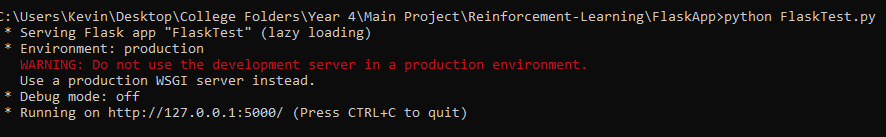
\includegraphics[width=1\linewidth]{img/flaskCmd}
	\caption{}
	\label{fig:flaskcmd}
\end{figure}
The user enters the address of http://127.0.0.1:5050 into their browser and a web page is severed from the root resource of the application with the simple message "hello world".\\\\
The following folder structure is used within a flask project.
\begin{minted}{python}
# The parent project folder
Root folder\
	# The main http routing script
	FlaskApp.py 
	# A python file that can be called
	PythonScript.py 
	# For deployment of application
	DeploymetFile.yaml
	# Declares the application python requirements at deploy time 
	RequirementsFile.txt 
	# For the staicly served files
	Static Folder\
		JavaScript Folder\
			file1.js
			filw2.js
			file3.js
		Css folder\
			style.css
		Data Folder\
			Data1.txt
			Data2.csv
			Data3.json
			Data4.xml
	# For the html templates sent back in the response body
	Templates Folder\
		home.html
		result.html
		pooling.html
\end{minted}

  
\section{REST Architecture}
The  Representational State Transfer Protocol (REST) is an architectural design philosophy that  is used to acquire resources held on a server via HTTP Requests/Responses. The REST architecture is know as stateless whereby the server holds no information about the clients session state. The session state is held locally by the client. The server only receives a client request, then sends a response back to the client with the resources requested. Resources can be in the form of text, image or html files etc. A client request is in the form of a URL with "address.com" being the physical address of the sever and "/resource-request" the actual resource needed to be sent back within the response body~\cite{Understa52:online}. 
\begin{minted}{HTTP}
https://address.com/resource-request
\end{minted} 
The main http request methods used within the REST architecture are:
\begin{itemize}
	\item GET should be used to retrieve an existing resource held on the server.
	\item POST should be used to create a resource on the server.
	\item PUT should be used to update a resource held on the server.
	\item DELETE should be used to remove a resource from the server.
\end{itemize}
Note that should is used in describing the four methods above.
As rest is not a standard but rather a set of guidelines to follow, the above methods can be used for different functionality but would not be considered a restful application.
\section{JavaScript}
JavaScript is a client side browser based scripting language.
It can be used to dynamically update information on a static web page in the form of tabular data, 2D/3D animations or session based user information~\cite{JavaScri52:online}, this will be discussed further in the following subsequent subsections. JavaScript can also be used to manipulate html elements with event listeners. In the below example~\cite{fontSize:online} an onClick event listener is used to change the font size of the text contained with the html paragraph element. The element is accessed by document.getElementById('demo'). This parses the document object model DOM of the html file and locates the element with the id of 'demo'. From here  ('demo').style.fontSize='35px' alters the text style font size to 35 pixels.
This is all done dynamically via a click event on the web page allowing for the local client side real time manipulation of browser data.
\begin{minted}{HTML}
<!DOCTYPE html>
<html>
<body>

<h2>What Can JavaScript Do?</h2>

<p id="demo">JavaScript can change the style of an HTML element.</p>

<button type="button" onclick="document.getElementById('demo')
                    .style.fontSize='35px'">Click Me!</button>

</body>
</html> 
\end{minted}  
\subsection{AJAX}
Asynchronous JavaScript and XML (AJAX) is a front end browser technology wich allows for the retrieval of server side data asynchronously without altering the view or behaviour of the web page. When an asynchronous request is made to the server it simply waits until a response has been returned and can then process the returned data. This method can be used to request specific files held on the server then run any data processing needed once the files have been returned.  AJAX also has the ability to only update partial segments of a web page without reloading the entire page.~\cite{AJAX:online}\\
In the below example~\cite{AJAXDemo:online} there is a h1 heading with the text "The XMLHttpRequest Object" along with a button holding an onClick event listener. When the button is clicked within the browser the loadDoc() JavaScript function is called.\\
Within the loadDoc function the onreadystatechange method waits for a http message of 4 and 200 response from the server which indicates the message has been sent correctly. From there the response text form the "ajax info" file is bound to the div with the id of demo changing the on screen text to the text held within the file.\\
 
\begin{minted}{HTML}
<!DOCTYPE html>
<html>
<body>

<div id="demo">
<h1>The XMLHttpRequest Object</h1>
<button type="button" onclick="loadDoc()">Change Content</button>
</div>

<script>
function loadDoc() {
var xhttp = new XMLHttpRequest();
xhttp.onreadystatechange = function() {
if (this.readyState == 4 && this.status == 200) {
document.getElementById("demo").innerHTML =
this.responseText;
}
};
xhttp.open("GET", "ajax_info.txt", true);
xhttp.send();
}
</script>

</body>
</html>
\end{minted}


\subsection{Google Charts}
The Google charts API is javaScript charting library that allows for the creation of numerous types of charts to be generated within a browser window. For the purpose of this project a line chart is used to display the agent rewards gained over time. Scalable Vector Graphics (SVG) are used to render the chart image within the browser~\cite{GoogleLineChart:online}.\\
To create a line chart:
\begin{itemize}
	\item The library must be imported along with an empty div to hold the final rendered image of the chart~\cite{GoogleLineChart:online}.

\end{itemize}

\begin{minted}{HTML}
<script type="text/javascript" src="https://www.gstatic.com/charts/loader.js">
</script>
<div id="chart_div"></div>
\end{minted}
\begin{itemize}
	\item The line chart package is loaded from the library.
	\item A callback function then used to load the drawBasic() function.
\end{itemize}
\begin{minted}{JavaScript}
google.charts.load('current', {packages: ['corechart', 'line']});
google.charts.setOnLoadCallback(drawBasic);
\end{minted}
The drawBasic() function has the following elements
\begin{itemize}
	\item A data table is first instantiated to hold all of the columns, rows and data. Then columns are created with declared data types and a name. ~\cite{GoogleLineChart:online}
\end{itemize}
\begin{minted}{JavaScript}
function drawBasic() {

var data = new google.visualization.DataTable();
data.addColumn('number', 'X');
data.addColumn('number', 'Dogs');

\end{minted}
\begin{itemize}
	\item The numerical data is then added to the data table as rows. The data is represented by a two dimensional JavaScript array~\cite{GoogleLineChart:online}.
\end{itemize}
\begin{minted}{JavaScript}
data.addRows([
[0, 0],   [1, 10],  [2, 23],  [3, 17],  [4, 18],  [5, 9],
[6, 11],  [7, 27],  [8, 33],  [9, 40],  [10, 32], [11, 35],
[12, 30], [13, 40], [14, 42], [15, 47], [16, 44], [17, 48],
[18, 52], [19, 54], [20, 42], [21, 55], [22, 56], [23, 57],
[24, 60], [25, 50], [26, 52], [27, 51], [28, 49], [29, 53],
[30, 55], [31, 60], [32, 61], [33, 59], [34, 62], [35, 65],
[36, 62], [37, 58], [38, 55], [39, 61], [40, 64], [41, 65],
[42, 63], [43, 66], [44, 67], [45, 69], [46, 69], [47, 70],
[48, 72], [49, 68], [50, 66], [51, 65], [52, 67], [53, 70],
[54, 71], [55, 72], [56, 73], [57, 75], [58, 70], [59, 68],
[60, 64], [61, 60], [62, 65], [63, 67], [64, 68], [65, 69]
]);
\end{minted}

\begin{itemize}
	\item Within the options object the chart can be customised. Below names are then given to the horizontal and vertical. axis~\cite{GoogleLineChart:online}
\end{itemize}
\begin{minted}{JavaScript}
 var options = {
hAxis: {
title: 'Time'
},
vAxis: {
title: 'Popularity'
}
};

\end{minted}
\begin{itemize}
	\item Finally the container div for the chart is identified and the chart.draw method is called with the data array and personalised options as parameter arguments.~\cite{GoogleLineChart:online}
\end{itemize}
\begin{minted}{JavaScript}
      var chart = new google.visualization.LineChart(
                  document.getElementById('chart_div'));

chart.draw(data, options);
\end{minted}
This will result in a rendered line chart SVG image to the browser.~\cite{GoogleLineChart:online}

\begin{figure}[H]
	\centering
	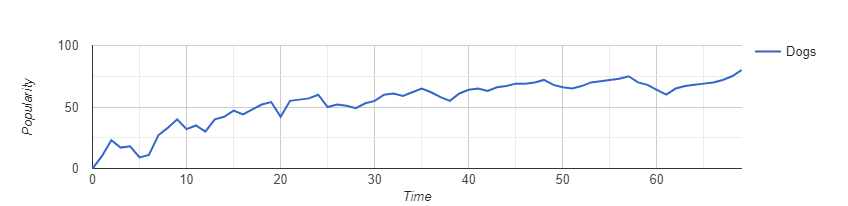
\includegraphics[width=0.7\linewidth]{img/goolgeChart}
	\caption{Goolge Line Chart}
	\label{fig:goolgechart}
\end{figure}

\subsection{Hottie heat mapping JavaScript Library}
Hottie is an open source heat mapping JavaScript library used to colour code data being generated. Any number of colour transitions can be used to represent low to high values within a dataset.The values in between low to high will have a gradient value based on the highest/ lowest value within the dataset.~\cite{HeatMap:online}\\
The hottie.js library is a used via JQuery and has the ability to colour code html tabular data based on the numerical values held within each table cell. The below example is a simple html table with some floating point values inserted into the table cells. The table has an ID of "myTable" for data access via JQuery.~\cite{HottieExample:online}
\begin{minted}{HTML}
<table id="myTable">
	<tr>
		<td>2.59</td><td>0.68</td><td>1.35</td>
		<td>1.35</td><td>2.03</td><td>1.60</td>
	</tr>
	<tr>
		<td>1.39</td><td>0.70</td><td>1.22</td>
		<td>1.08</td><td>1.00</td><td>2.12</td>
	</tr>
	<tr>
		<td>2.87</td><td>0.59</td><td>1.22</td>
		<td>0.57</td><td>1.08</td><td>3.00</td>
	</tr>
	<tr>
		<td>0.99</td><td>0.25</td><td>0.48</td>
		<td>0.50</td><td>0.99</td><td>1.77</td>
	</tr>
</table>
\end{minted}
Using JQuery a handle is gained on the table via the ID of "myTable". Three transitional hex colour values are then set from low (red), medium (red + green) to high (green).~\cite{HottieExample:online}
\begin{minted}{JavaScript}
$("#myTable td").hottie({
colorArray : [ 
"#63BE7B",
"#FBE983",
"#F8696B"
]
});
\end{minted}
The resulting cell values within the html table now have colour codes mapped to them based on the lowest (red) to highest (green) values. Every value in between the lower and upper bound will have a mixture of the two colours. The amount of colour mix is dependant on the current value within the cell and how close it is to the lowest/highest value.~\cite{HeatMap:online}~\cite{HottieExample:online}\\
\begin{figure}[H]
	\centering
	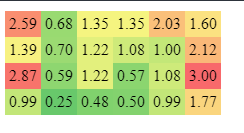
\includegraphics[width=0.7\linewidth]{img/HeatMap}
	\caption{}
	\label{fig:heatmap result}
\end{figure}

\subsection{HTML Canvas}
The html canvas element is used to draw graphics via JavaScript and render the result within a browser page.\\
All of the drawing commands are written in JavaScript then sent to the empty canvas element for the resulting image to be rendered by the browser.\\
Below is a simple example of a line drawn using html canvas.~\cite{CanvasDoc:online}\\
The attributes the canvas element have are the with and height of the canvas view, the ID and optional styling if needed~\cite{CanvasExample:online}.

\begin{minted}{HTML}
<canvas id="myCanvas" width="200" 
           height="100" style="border:1px solid #000000;">
</canvas>
\end{minted}
To draw the line firstly a handle is gain on the canvas element with the ID of "myCanvas".\\
The context of the canvas is then declared as a two dimensional drawing.\\
The moveTo() method tells the browser where to start the drawing with 0,0 being the x,y coordinates.
The x,y coordinates 0,0 start at the top left of the canvas which is not the conventional position of bottom left.\\
The lineTo() method states where to draw a line along the x,y coordinates. In the below example a line is drawn 200 pixels along the x axis and 100 pixels along the y axis giving the result of a diagonal line from the top left to the bottom right of the containing canvas.~\cite{CanvasExample:online,CanvasDoc:online}
\begin{minted}{JavaScript}
var c = document.getElementById("myCanvas");
var ctx = c.getContext("2d");
ctx.moveTo(0, 0);
ctx.lineTo(200, 100);
ctx.stroke();
\end{minted}
\begin{figure}[H]
	\centering
	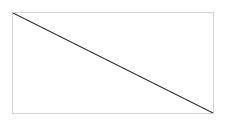
\includegraphics[width=0.7\linewidth]{img/canvasLine}
	\caption{}
	\label{fig:canvasline}
\end{figure}

\section{Bootstrap} 
Bootstrap is a CSS framework library that allows for the rapid development of a fully responsive front end user interface.\\
All css is pre-written with pre-defined class/id names.\\
To utilise the BootStrap framework all that is required is to assign the html elements a class name or ID matching the class names or ID within the Bootstrap CSS file~\cite{Bootstrap:online}.
In the below example a simple grid layout is used by declaring three types of div with the class names of:
\begin{itemize}
	\item "container" the wrapper class that controls the responsiveness of all containing divs.
	\item "row" the class that identifies a section of the horizontal view within the browser.
	\item "col-sm" the class that identifies each column. col-sm is used in this example but the width can be set by adding a value at the end of the class name. col-sm-12 will give the column a full width of the browser window. If no numeric value is given the column width is decided by dividing the number of col class names by 12. In the below example each column is assigned a width of four as there are three divs with the class name of "col-sm".
\end{itemize} 

\begin{minted}{HTML}
<div class="container">
	<div class="row">
		<div class="col-sm">
		One of three columns
		</div>
		<div class="col-sm">
		One of three columns
		</div>
		<div class="col-sm">
		One of three columns
		</div>
	</div>
</div>
\end{minted}

The above BootStrap html will produce the following result in a browser view on a desktop at full screen~\cite{BootstrapGridExample:online}.
\begin{figure}[H]
	\centering
	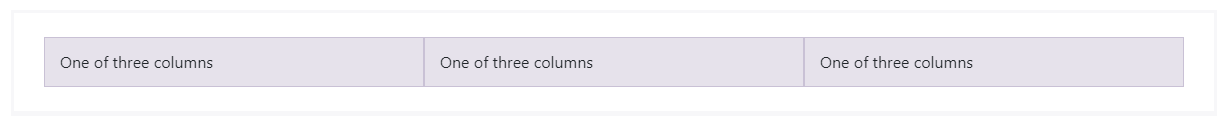
\includegraphics[width=0.7\linewidth]{img/BootstrapFullScreen}
	\caption{}
	\label{fig:bootstrapfullscreen}
\end{figure}

The below image is a view of the same BootStrap html viewed on a mobile device~\cite{BootstrapGridExample:online}.
\begin{figure}[H]
	\centering
	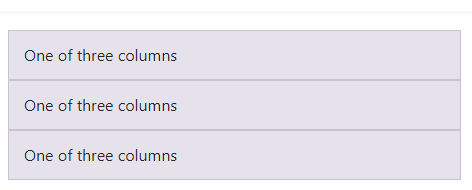
\includegraphics[width=0.7\linewidth]{img/BootstrapMobile}
	\caption{}
	\label{fig:bootstrapmobile}
\end{figure}

\section{Json}
JavaScript Object Notation (Json) is a language independent text based representation of a data object. This allows for the marshalling and un-marshalling of data to an object across many different programming languages. The Json data is written to a file with the .json extension and usually held on a server. The .json file contents are plain text, which are interpreted by a programming language requesting the file from the server. Once the file has been received the data can be un-marshalled to the language specific object~\cite{JSON:online}. In the below example a JavaScript object will be used to explain the process.\\

The .json file structure has  a parent container node named performance. Within this parent node there are two child nodes with key value pairs. The key for each object is named timeStep and reward with numerical values as the value for each key.~\cite{JSONstring:online}\\
\begin{minted}{JSON}
{"Performance":[
{ "timeStep":1, "reward":45 },
{ "timeStep":2, "reward":100 }
]}
\end{minted}
When the file is requested from the server it needs to be parsed so it can be read as a JavaScript object.

\begin{minted}{JavaScript}
var obj = JSON.Parse(demo.json);
\end{minted}
The variable obj is now converted to a JavaScript object array and can be used as needed within the browser to display the relevant data.
\begin{minted}{JavaScript}
["Performance",
 [
  "timeStep"
   [
    1
   ]
 ],
 [
  "reward"
   [
    45
   ]
 ],
 [
  "timeStep"
   [
    2
   ]
 ],
 [
  "reward"
   [
    100
   ]
 ]
]
\end{minted}
\section{CSV}
A Comma Separated Value (CSV) file is used for storing data in a tabular format. Each new line within the file represents a new data entry. CSV files can be used to store multiple data types within the same file. It is then up to the program opening the file to interpret the data as needed. Below is a simple example of some numerical data entries within a csv file.~\cite{CSVPython:online} 

\begin{minted}{JavaScript}
	1,30,80,300
	2,59,67,-59
	3,40,22,21
\end{minted}

To parse this data an ajax call to a server can be used to request the file needed.~\cite{ParsingCSVExample:online}
\begin{minted}{Javascript}
$.ajax({
  type: "GET",
  url: "static/Data/test.csv",
  dataType: "text",
  cache: false,
  async: true,
  success: function(data) {
    // Array of data
    var data =data;

    $('table').append('<tr class="data"><td>'+data[0] + 
              '</td><td>'+data[1]+'</td><td>'+data[2] +
              '</td><td>'+data[3]+'</td></tr>');

  }

});
\end{minted}
In the above example once the csv file has been received from the server the data is placed into an array and appended to a html table for rendering the data to the browser page within a table cells~\cite{ParsingCSVExample:online}.
\section{Google Cloud App Engine}
The Goolge Cloud app engine is used to deploy and host web applications to a live server.\\
In the below example a python flask application is used, however a number of different languages can be used for deployment.\\
The following requirements are needed to deploy an application to Goolge Cloud App Engine.
\begin{itemize}
	\item Create App Engine instance:
	A new project is needed as a container for the application~\cite{CreatingAppEngine:online}.
	\begin{figure}[H]
		\centering
		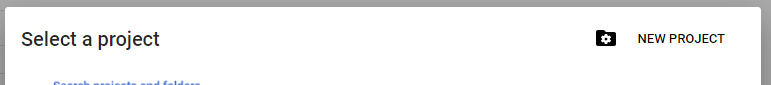
\includegraphics[width=0.7\linewidth]{img/GoogleNEwPRoject}
		\caption{}
		\label{fig:googlenewproject}
	\end{figure}
	
	\item A locally created Flask project as discussed within the flask section of this chapter.
	\item app,yaml file:
	This file contains the configuration settings for the application declaring the programming language, Version number, libraries used, static directories and the main flask file name~\cite{FlaskAppGoolge:online}.
\begin{minted}{yaml}
runtime: python27
api_version: 1
threadsafe: true

libraries:
- name: ssl
version: latest

handlers:
- url: /static
static_dir: static
- url: /.*
script: main.app
\end{minted}
	\item requiremets.txt file:
	This file declares the different dependencies that are needed for the application to run.
	In the below example the flask and Werkzeug versions are declared~\cite{FlaskAppGoolge:online}.
\begin{minted}{text}
Flask==0.12.4
Werkzeug<0.13.0,>=0.12.0
\end{minted}
	\item Google Cloud SDK:
	The Google SDK must be installed locally to enable the deployment of the project to the app engine. Once the SDK has been installed open the command line tool and change to the root directory of the project folder. Once inside the directory type the following command to deploy the application~\cite{FlaskAppGoolge:online}.
\end{itemize}
\begin{figure}[H]
	\centering
	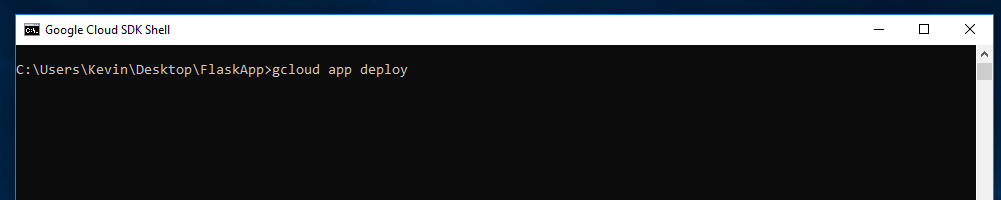
\includegraphics[width=0.7\linewidth]{img/DeployCmd}
	\caption{}
	\label{fig:deploycmd}
\end{figure}
Once the deployment has completed the application will be available at appname.appspot.com. ~\cite{FlaskAppGoolge:online}


\chapter{System Design}
This chapter will examine the overall architecture and individual system components. These will be discussed at a high level view for the main structure of the system. The major functional components will then be broken down into a more fine grain view for examination. In addition the interaction between the components will be explained in further detail.

\section{System Architecture}
This system is client server based architecture with all of the system resources held on a server. The client interacts with the server via a resource http requests. When the client first enters the root URL of the application address a request is made for the "Index.hmtl" web page. If found the index page along with any other JavaScript or CSS files are sent back to the browser for rendering.

\begin{figure}[H]
	\centering
	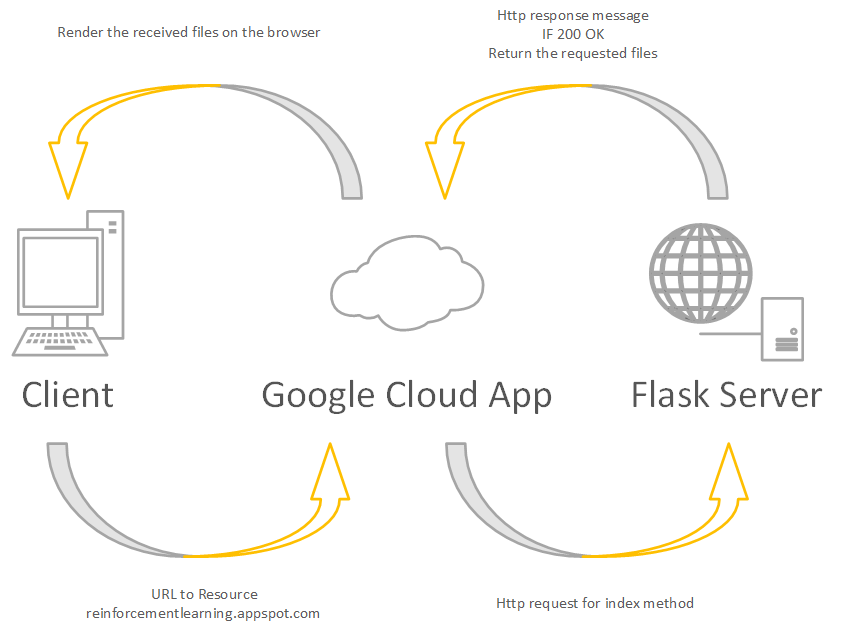
\includegraphics[width=0.7\linewidth]{img/Architecture}
	\caption{Architectural Diagram}
	\label{fig:architecture}
\end{figure}

In the following images the server will be launched locally. A request will be then sent to the server for the root resource. Finally the home page will be sent back to the browser to render the page to the user.

\begin{figure}[H]
	\centering
	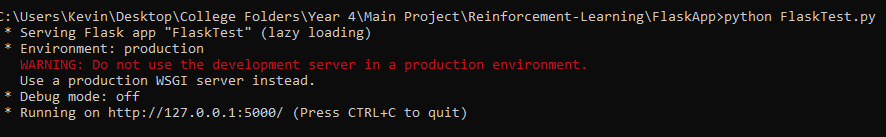
\includegraphics[width=0.9\linewidth]{img/flaskCmd}
	\caption{Starting the server}
	\label{fig:flaskcmd}
\end{figure}
The above image is the flask server running and listening for requests at http://127.0.0.1:5000/.\\
Once the URL has been entered to the address bar of the browser. 
The resource root method is called in the main Flask server file.
\begin{minted}{Python}
@app.route('/')
def index():
# Return the main home page when the route resource is requested
return render_template('index.html')
\end{minted}
The above root method returns the index.hmtl file within the response body to be read by the browser.

If everything is ok and all resources can be retrieved a status message of 200 is sent to the browser.
\begin{figure}[H]
	\centering
	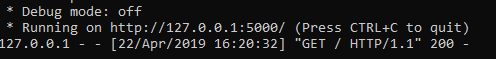
\includegraphics[width=0.9\linewidth]{img/http200}
	\caption{http 200}
	\label{fig:http200}
\end{figure}

Finally the home page is rendered to the user.
\begin{figure}[H]
	\centering
	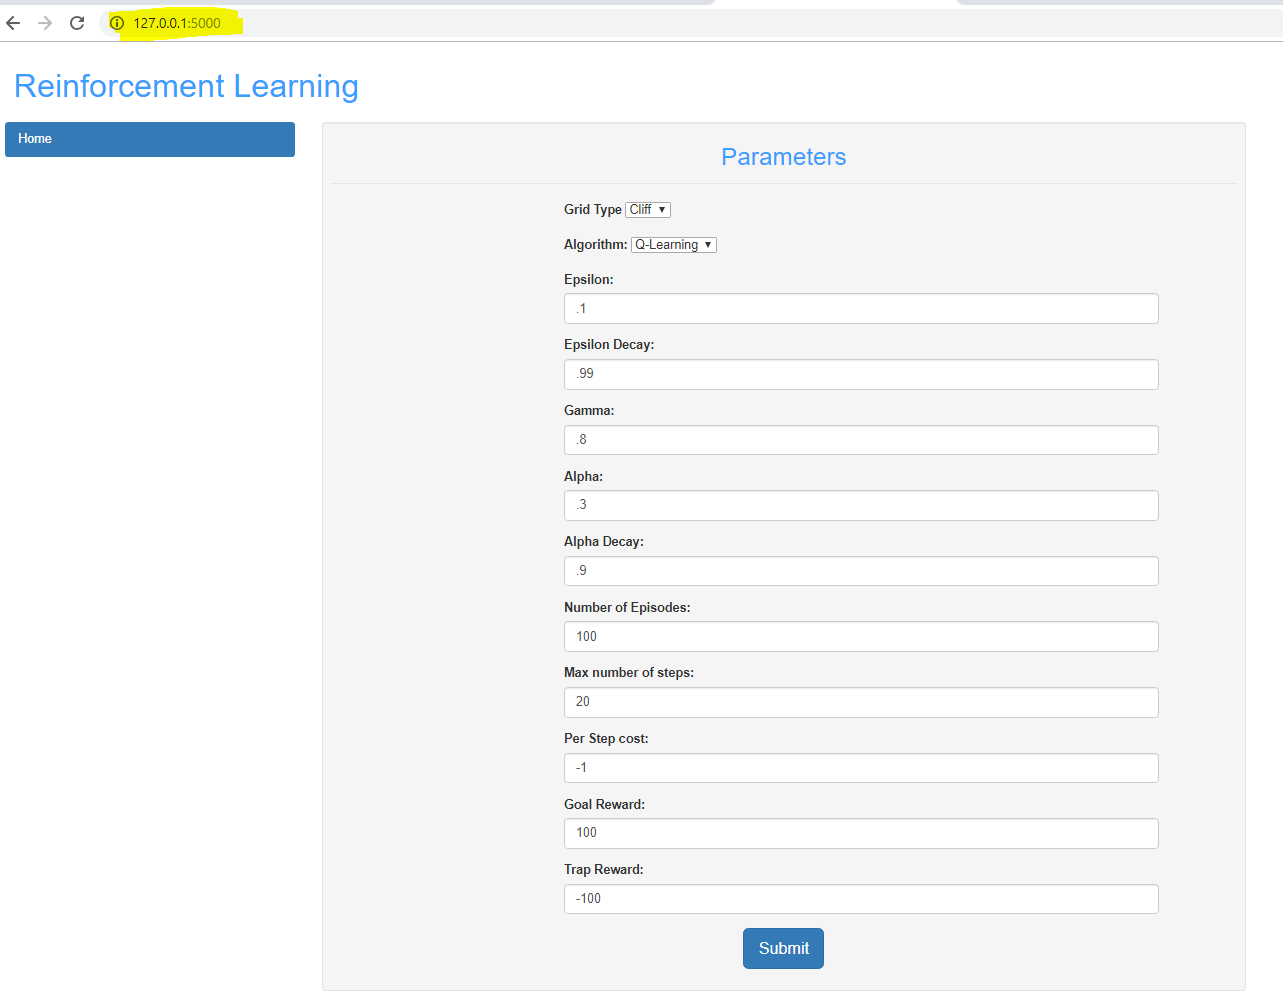
\includegraphics[width=0.9\linewidth]{img/homePage}
	\caption{Rendered Home Page}
	\label{fig:homepage}
\end{figure}
When the highlighted url is entered to the browser address. The index html page is sent back to the browser along with any CSS and JAvaScript files needed.

This example is a brief introduction of the overall architecture of the application. A more in depth investigation of each system component will be discussed in the next chapter.

\section{System Components}

\section{Component Interaction}

\section{Data Flow}

\section{deployment}



\chapter{System Evaluation}
As many pages as needed.
\begin{itemize}
\item Prove that your software is robust. How? Testing etc. 
\item Use performance benchmarks (space and time) if algorithmic.
\item Measure the outcomes / outputs of your system / software against the objectives from the Introduction.
\item Highlight any limitations or opportunities in your approach or technologies used.
\end{itemize}

\chapter{Conclusion}
About three pages.

\begin{itemize}
\item Briefly summarise your context and ob-jectives (a few lines).
\item Highlight your findings from the evalua-tion section / chapter and any opportuni-ties identified.
\end{itemize}

